\documentclass{is2014}

%----------------------------------------------------------------------------------------
%	PACKAGES AND OTHER DOCUMENT CONFIGURATIONS
%----------------------------------------------------------------------------------------

\usepackage{lineno}% Use line numbers
\modulolinenumbers[1]

%----------------------------------------------------------------------------------------
%	TITLE SECTION
%----------------------------------------------------------------------------------------

\title{Title of the Talk} % The title here

\author{
  A. Author \\ 
  University of California, Berkeley, CA 94720 \\
%%  \and
%%  B. Buthor, for the ALICE Collaboration \\
%%  LBNL, Berkeley, CA 94720 \\
  \vspace{-5mm}
}

\date{}

%----------------------------------------------------------------------------------------

\begin{document}
\linenumbers %% Comment before submitting to arXiv

\maketitle % Insert title

\thispagestyle{fancy} % All pages have headers and footers

%----------------------------------------------------------------------------------------
%	ABSTRACT
%----------------------------------------------------------------------------------------

\begin{abstract}

\noindent 
\lipsum[1] % Dummy abstract text

\end{abstract}

%----------------------------------------------------------------------------------------
%	ARTICLE CONTENTS
%----------------------------------------------------------------------------------------

\begin{multicols}{2} % Two-column layout throughout the main article text

\section{Introduction}

\lipsum[2-3] % Dummy text

%------------------------------------------------

\section{Methods section with list}

Maecenas sed ultricies felis. Sed imperdiet dictum arcu a egestas. 
\begin{compactitem}
\item Donec dolor arcu, rutrum id molestie in, viverra sed diam
\item Curabitur feugiat
\item turpis sed auctor facilisis
\item arcu eros accumsan lorem, at posuere mi diam sit amet tortor
\item Fusce fermentum, mi sit amet euismod rutrum
\item sem lorem molestie diam, iaculis aliquet sapien tortor non nisi
\item Pellentesque bibendum pretium aliquet
\end{compactitem}
\lipsum[4] % Dummy text

%------------------------------------------------

\section{Results}

\subsection{A subsection with a Table and Equation}

\begin{table}[H]
\caption{Example table}
\centering
\begin{tabular}{llr}
\toprule
\multicolumn{2}{c}{Name} \\
\cmidrule(r){1-2}
First name & Last Name & Grade \\
\midrule
John & Doe & $7.5$ \\
Richard & Miles & $2$ \\
\bottomrule
\end{tabular}
\end{table}

\lipsum[5] % Dummy text
\begin{equation}
\label{eq:emc}
e = mc^2
\end{equation}

\subsection{A subsection with a Figure}
\lipsum[6] % Dummy text
\begin{figure}[H]
   \centering
   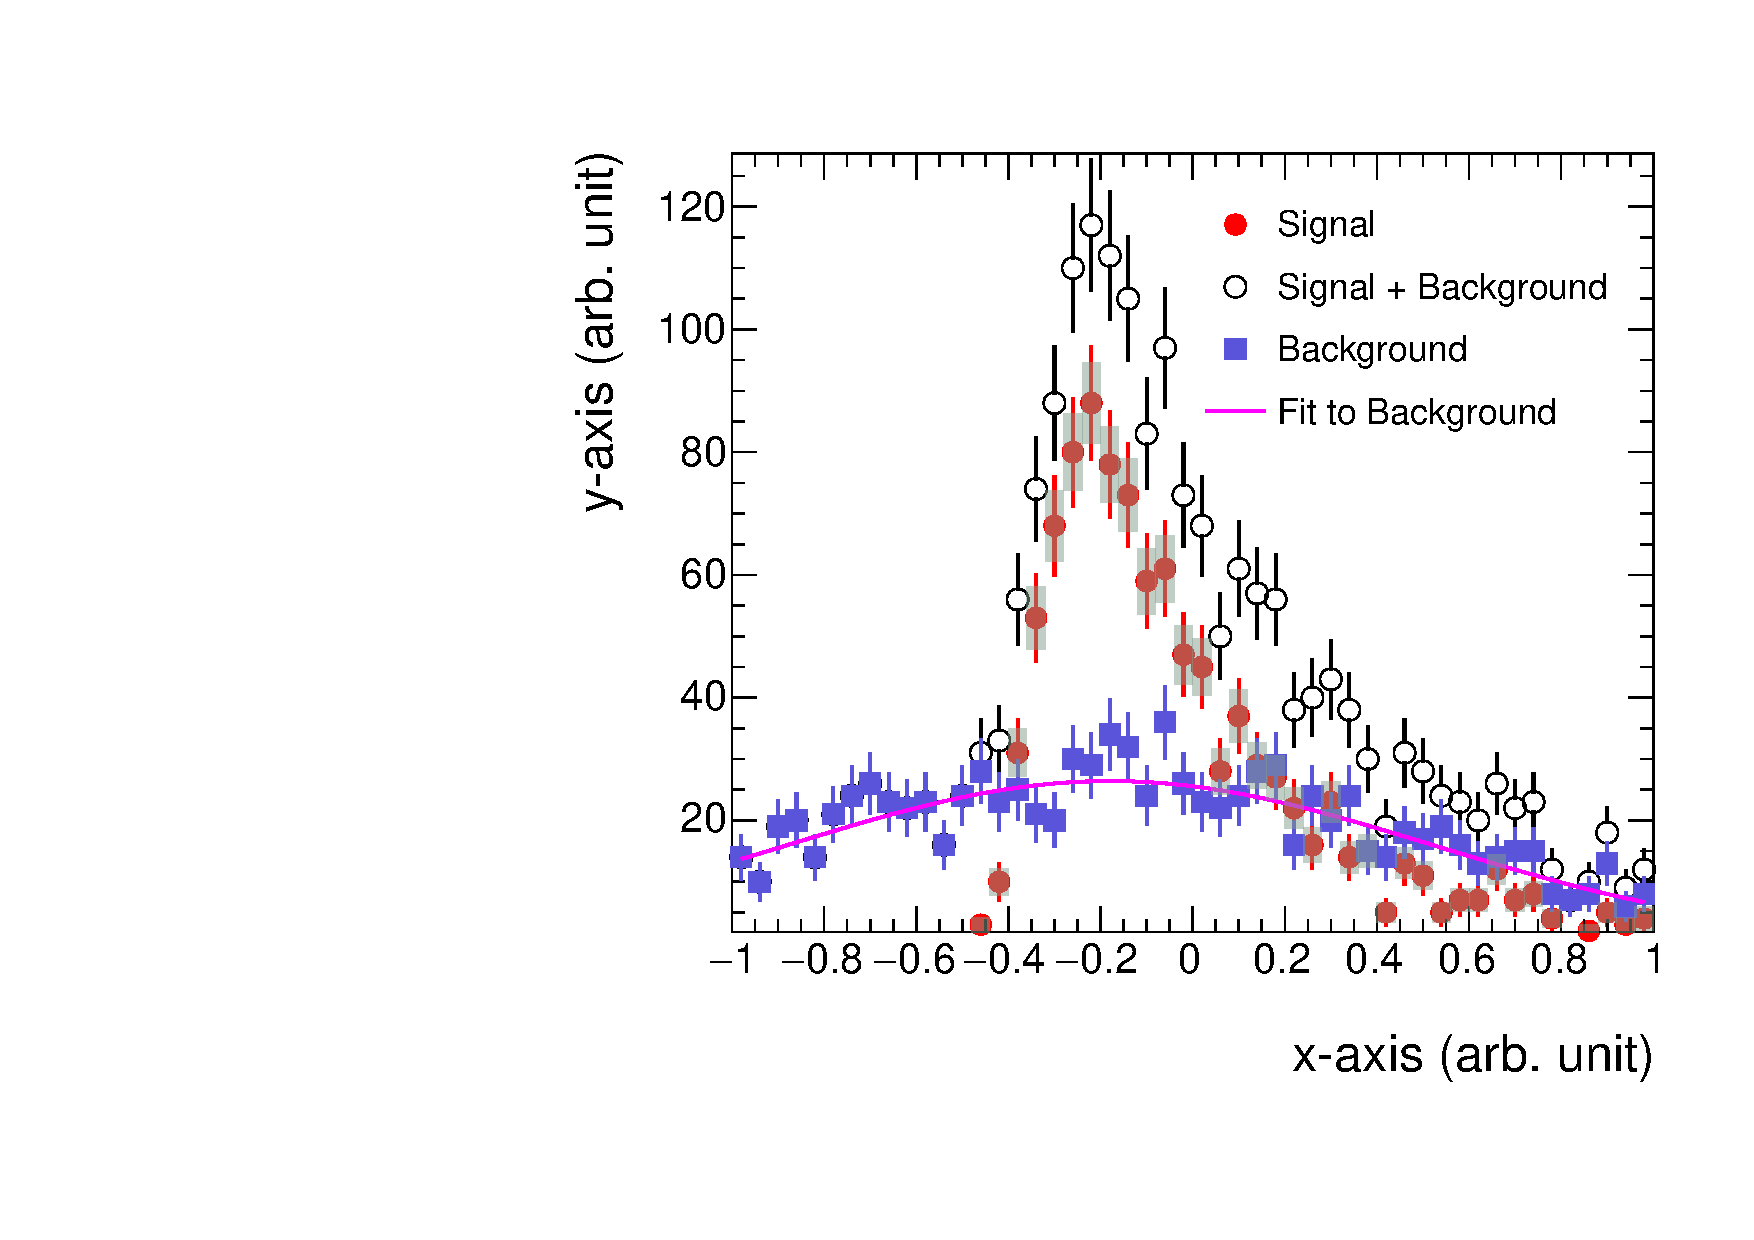
\includegraphics[width=0.45\textwidth]{example-plot-canvas.pdf} % requires the graphicx package
   \caption{Caption to the example plot.}
   \label{fig:example}
\end{figure}
\lipsum[7] % Dummy text
Here we refer to Fig. \ref{fig:example}.

%----------------------------------------------------------------------------------------
%	REFERENCE LIST
%----------------------------------------------------------------------------------------

\begin{thebibliography}{99} % Bibliography - this is intentionally simple in this template

\bibitem{Figueredo:2009dg}
Figueredo, A.~J. and Wolf, P. S.~A. (2009).
\newblock Assortative pairing and life history strategy - a cross-cultural
  study.
\newblock {\em Human Nature}, 20:317--330.
 
\end{thebibliography}

%----------------------------------------------------------------------------------------

\end{multicols}

\end{document}
